\section{Aufgabenstellung und Versuch}

Aus den bereits aufgestellten DGL-System kann das Blockschaltbild in Simulink
erstellt werden.

\begin{figure}[H]
    \centering
    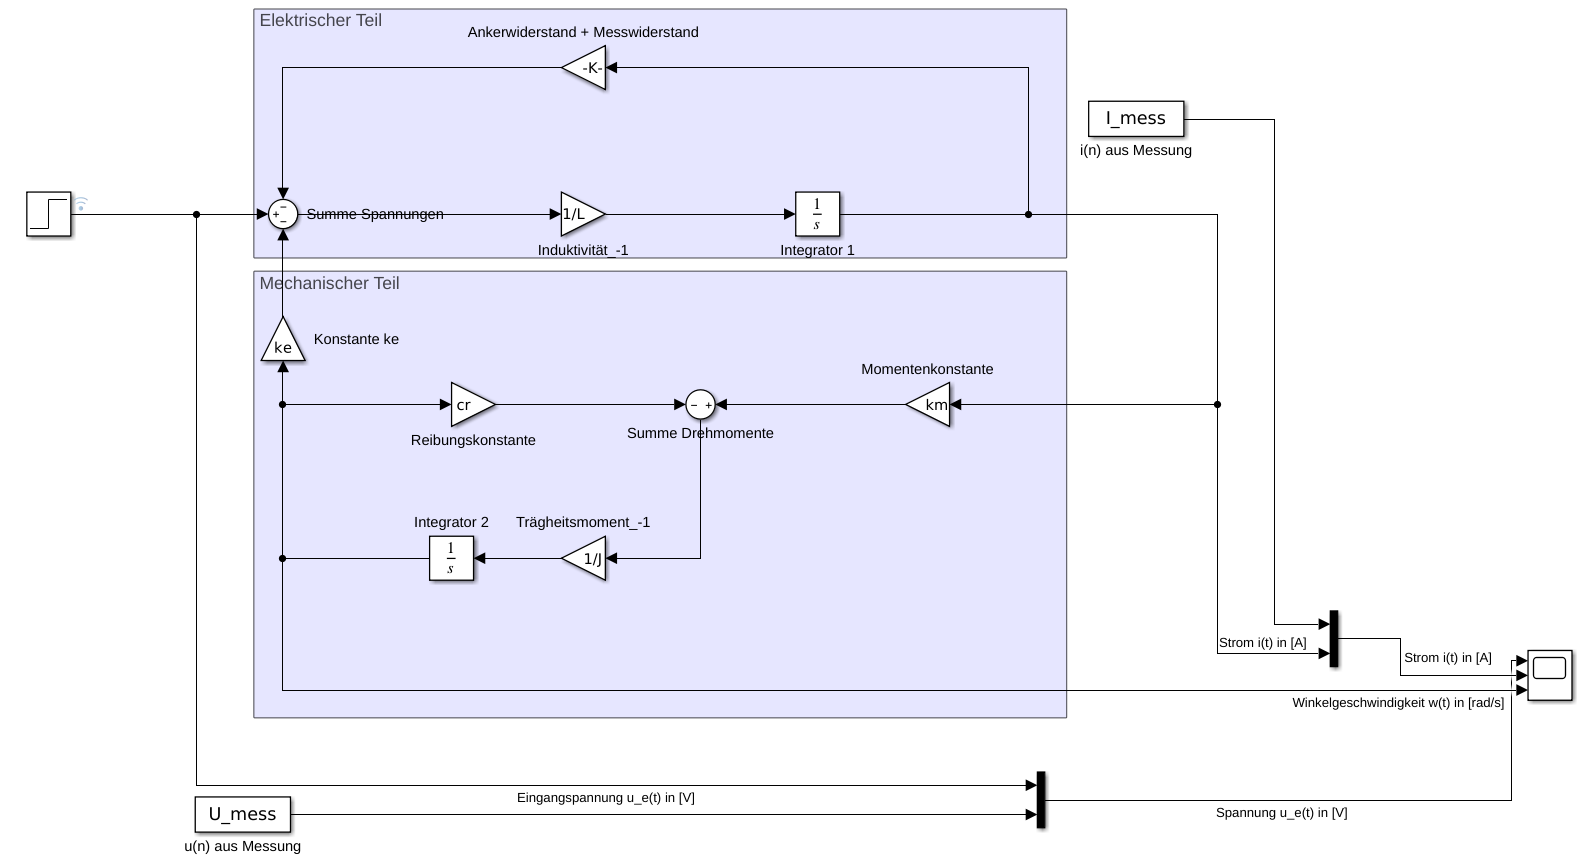
\includegraphics[width=1\textwidth]{sl_modell.png}
    \caption{Blockschaltbild in Simulink}
    \label{fig:Blockschaltbild}
\end{figure}

Als Eingang wurde ein Step-Block benutzt und als Ausgang ein Scope-Block.
Die erste DGL wurden im oberen Teil des Modell realisiert und beschreibt
den elektrischen Teil des Systems. Im unteren wird der mechanische Teil
des Motors modelliert der aus der zweiten DGL hervorgeht.\\

Die schon ermittelten Konstanten des Systems wurden in einem Matlab-File
abgespeichert und werden über dieses auch aufgerufen. Auch die Daten der
Messung des Spungs und der Sprungantwort sind hier zufinden.\\

Um den gemessenen Spung und die Sprungantwort in Simulink anzuzeigen wurde der Block
"From Workspace" benutzt der jeweils den Zeit-Spannungs-Vektor und den Zeit-
Spannungs-Vektor lädt.\\

Der Spung aus dem Modell wurden dem Sprung aus der Messung mit folgenden
Parameter angepasst.\\

\begin{figure}[H]
    \centering    
    \begin{tabular}[h]{l| r}
        Steptime & 0.048s \\
        \hline
        Final Value & 8.2V \\
        \hline
        Sampletime & 0.001s \\
    \end{tabular}
    \caption{Parameter Step Block}
\end{figure}
    

Um das Trägheitsmoment $J$ zu bestimmen, wurde dann $J$ auf den Initialwert
von $10^{-3}\mathrm{Kg \cdot m^2}$ gesetzt. Dieser stammt aus dem Datenblatt
des DCX10L aus der Vorlesung.

Danach haben wir das System für 30 Sekunden simuliert und erhielten folgendes
Ergebnis.

\begin{figure}[H]
    \centering
    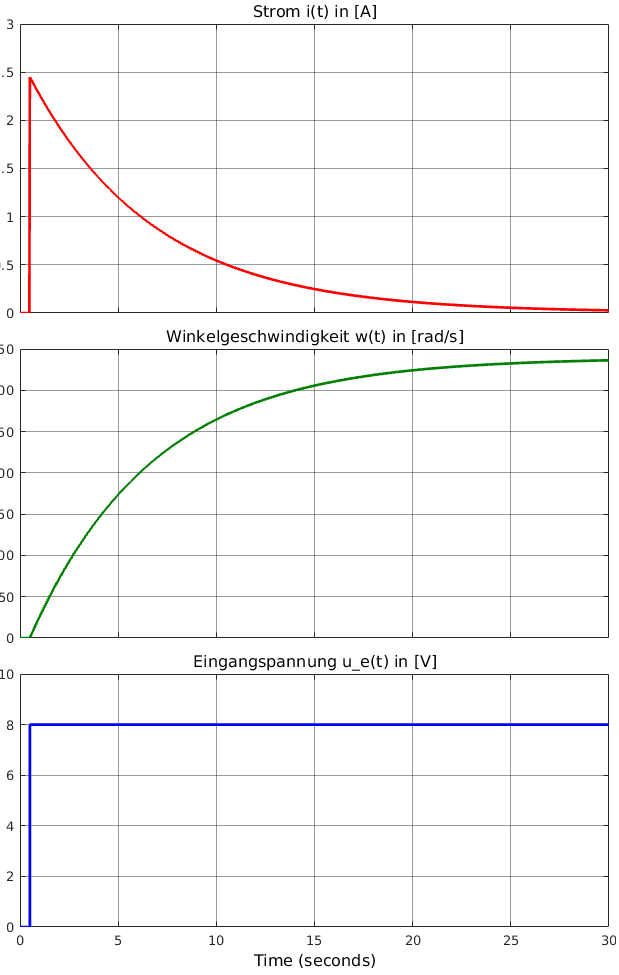
\includegraphics[width=0.75\textwidth]{data_modell.png}
    \caption{Simulation 1}
    \label{fig:Simulation 1}
\end{figure}

Wir haben dann durch manuelles iteratives Anpassen den Wert des Trägheitsmoments
so bestimmt, dass die Funktion des Modells mit den Messdaten übereinstimmt. 

\begin{equation} \label{eq311}
    \begin{split}
        J \simeq 5 \mathrm{\mu Kg \cdot m^2}
    \end{split}
\end{equation}

Anschließend simulierten wir in der Zeit der gegebenen Messdaten  $\Delta T= 0.6s$.
Daraus ergab sich folgendes Ergebnis.

\begin{figure}[H]
    \centering
    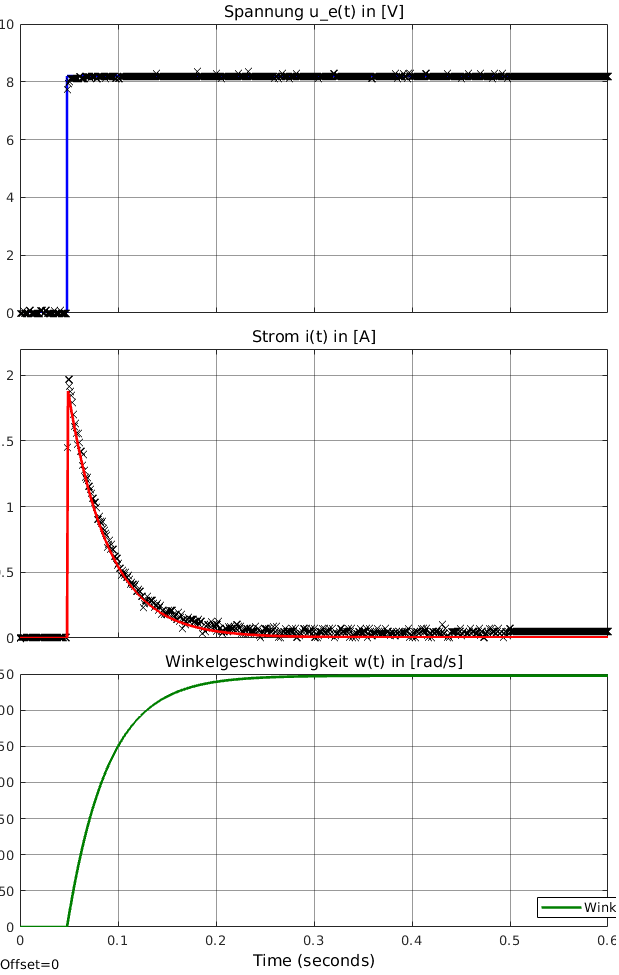
\includegraphics[width=0.75\textwidth]{data_modell_final.png}
    \caption{Simulation 2}
    \label{fig:Simulation 2}
\end{figure}